\documentclass[a4paper]{article}
\usepackage[english]{babel}
\usepackage{setspace}
\usepackage{mathtools}
\usepackage{listings}
\usepackage{ulem}
\usepackage[utf8]{inputenc}
\usepackage{eurosym}
\usepackage{fancyhdr}
\usepackage{tikz}
\usetikzlibrary{calc}
\usetikzlibrary{positioning}
\usetikzlibrary{arrows.meta}
\usetikzlibrary{fit}
\usepackage{tikzscale}
\usepackage{wrapfig}
\setcounter{secnumdepth}{-1}
\pagestyle{fancy}
\fancyhf{}
\lhead{Multi-Agent Systems, Exercise 1}
\cfoot{\thepage}
\begin{document}
\title{Exercise Sheet 1: Solution}
\author{}
\date{\today}
\section{Exercise 1.1}
\subsection{a)}
Each clause is a disjunction containing at least one negated atom. Therefore, the interpretation $p_i \mapsto \top \quad \forall i$ satisfies S.
\subsection{b)}
\begin{align*}
&(p \land (q \lor \lnot p))\lor(r \land \lnot(s \lor r)) \quad& \text{ Commutativity}\\
\implies&(p \land (\lnot p \lor q))\lor(r \land \lnot(r \lor s)) & \text{De Morgan}\\
\implies&(p \land (\lnot p \lor q))\lor(r \land \lnot r \land \lnot s)) & \text{Contradiction}\\
\implies&(p \land (\lnot p \lor q))\lor(\bot \land \lnot s)) & \text{Falsity}\\
\implies&(p \land (\lnot p \lor q))\lor\bot & \text{Falsity}\\
\implies& p \land (\lnot p \lor q) & \text{Distributivity}\\
\implies&(p \land \lnot p) \lor (p \land q) & \text{Contradiction}\\
\implies&\bot \lor (p \land q) & \text{Falsity}\\
\implies& p \land q & \\
\end{align*}
\section{Exercise 1.2}
\subsection{a)}
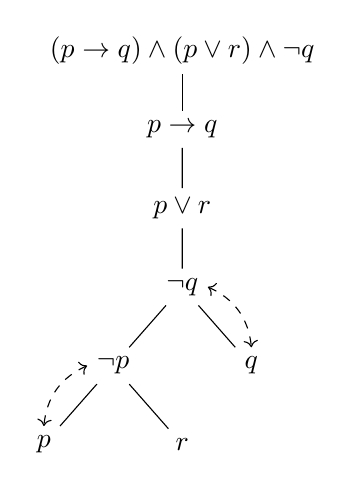
\begin{tikzpicture}[level distance=10mm,sibling distance=5em,every node/.style = {align=center}]
\node {$(p \rightarrow q) \land (p \lor r) \land \lnot q$}
    child { node {$p \rightarrow q$}
        child { node {$p \lor r$}
            child { node (a1) {$\lnot q$}
                child { node (b1) {$\lnot p$}
                    child { node (b2) {$p$}}
                    child { node {$r$}}}
                child { node (a2) {$q$}
}}}};
\draw [<->, dashed] (a1.east) to [bend left] (a2.north);
\draw [<->, dashed] (b1.west) to [bend right] (b2.north);
\end{tikzpicture}\\\\
All branches are either saturated or closed. The only open branch provides the model
$p \mapsto F, q \mapsto F, r \mapsto T$.
\subsection{b)}
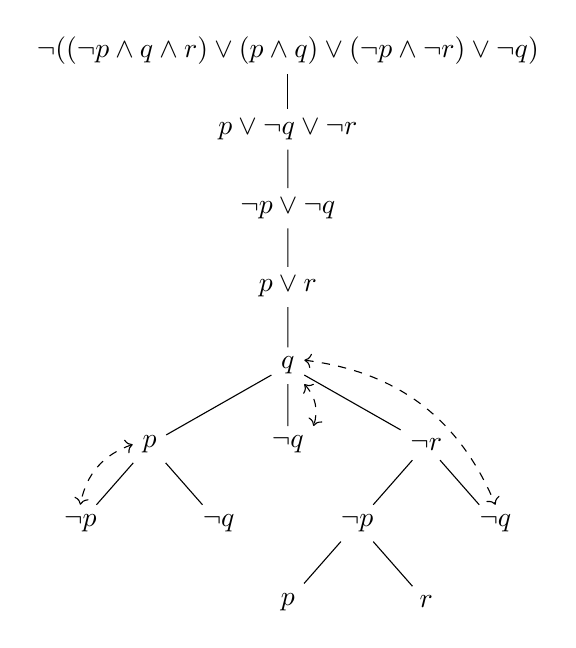
\begin{tikzpicture}[level distance=10mm,sibling distance=5em,every node/.style = {align=center}]
\node {$\lnot ((\lnot p\land q \land r) \lor (p \land q) \lor (\lnot p \land \lnot r) \lor \lnot q)$}
        child { node {$p \lor \lnot q \lor \lnot r$}
            child { node { $\lnot p \lor \lnot q$}
                child { node { $p \lor r$}
                    child { node (a1) {$q$}
                        child { node (b1) {$p$}
                            child { node (b2) {$\lnot p$}}
                            child { node {$\lnot q$}}}
                        child { node (a2) {$\lnot q$}}
                        child { node {$\lnot r$}
                            child { node {$\lnot p$}
                                child{ node {$p$}}
                                child{ node {$r$}}}
                            child { node (a3) {$\lnot q$}}}
}}}};
\draw [<->, dashed] (a1.south east) to [bend left] (a2.north east);
\draw [<->, dashed] (a1.east) ++(0, 0.2em) to [bend left] (a3.north);
\draw [<->, dashed] (b1.west) to [bend right] (b2.north);
\end{tikzpicture}\\\\
Since its negation is unsatisfiable, $(\lnot p\land q \land r) \lor (p \land q) \lor (\lnot p \land \lnot r) \lor \lnot q$ is a tautology.
\subsection{c)}
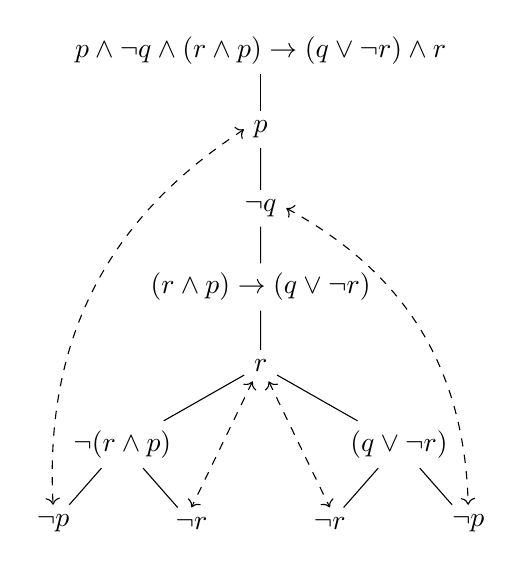
\begin{tikzpicture}[level distance=10mm,sibling distance=5em,every node/.style = {align=center},
level 5/.style={sibling distance=10em},
level 6/.style={sibling distance=5em}]
\node {$p \land \lnot q \land (r \land p) \rightarrow (q \lor \lnot r) \land r$}
    child { node (a1) {$p$}
        child { node (b1) {$\lnot q$}
            child { node {$(r \land p) \rightarrow (q \lor \lnot r)$}
                child { node (c1) {$r$}
                    child { node {$\lnot (r \land p)$}
                        child{ node (a2) {$\lnot p$}}
                        child{ node (c2) {$\lnot r$}}}
                    child { node {$(q \lor \lnot r)$}
                        child{ node (c3) {$\lnot r$}}
                        child{ node (b2) {$\lnot p$}}}
}}}};
\draw [<->, dashed] (a1.west) to [bend right] (a2.north);
\draw [<->, dashed] (b1.east) to [bend left] (b2.north);
\draw [<->, dashed] (c1.south west) ++(0.3em, 0) to (c2.north);
\draw [<->, dashed] (c1.south east) ++(-0.3em, 0) to (c3.north);
\end{tikzpicture}\\\\
$p \land \lnot q \land (r \land p) \rightarrow (q \lor \lnot r) \land r$ is unsatisfiable, therefore\\
$\{p \land \lnot q, (r \land p) \rightarrow (q \lor \lnot r)\} \models r$
\end{document}












